\documentclass[11pt]{article}

\title{Monte Carlo Simulations}
\author{David Kun}

\usepackage{amsmath}
\usepackage{graphicx}
\usepackage[pdftex]{hyperref}
\usepackage{amssymb}
\usepackage{color}
\usepackage[margin=0.5in]{geometry}

\begin{document}

% Title
\maketitle

% Content

\section*{Section 1}
In the first three cases, the leader and follower have the \emph{same} error covariance matrices, so:
\begin{align*}
Q_{(l)} &= Q_{(f)} = Q \\
R_{(l)} &= R_{(f)} = R \\
\text{where, } Q &: \text{state covariance error}\\
 R &: \text{sensor covariance error} \\
 \gamma &>1
\end{align*}
The cases that were tested in this section are:
\begin{itemize}
\item $Q=R$
\item $Q=R \times \gamma$
\item $Q=R \times \frac{1}{\gamma}$
\end{itemize}

\begin{figure}[!hbtp]
\centering
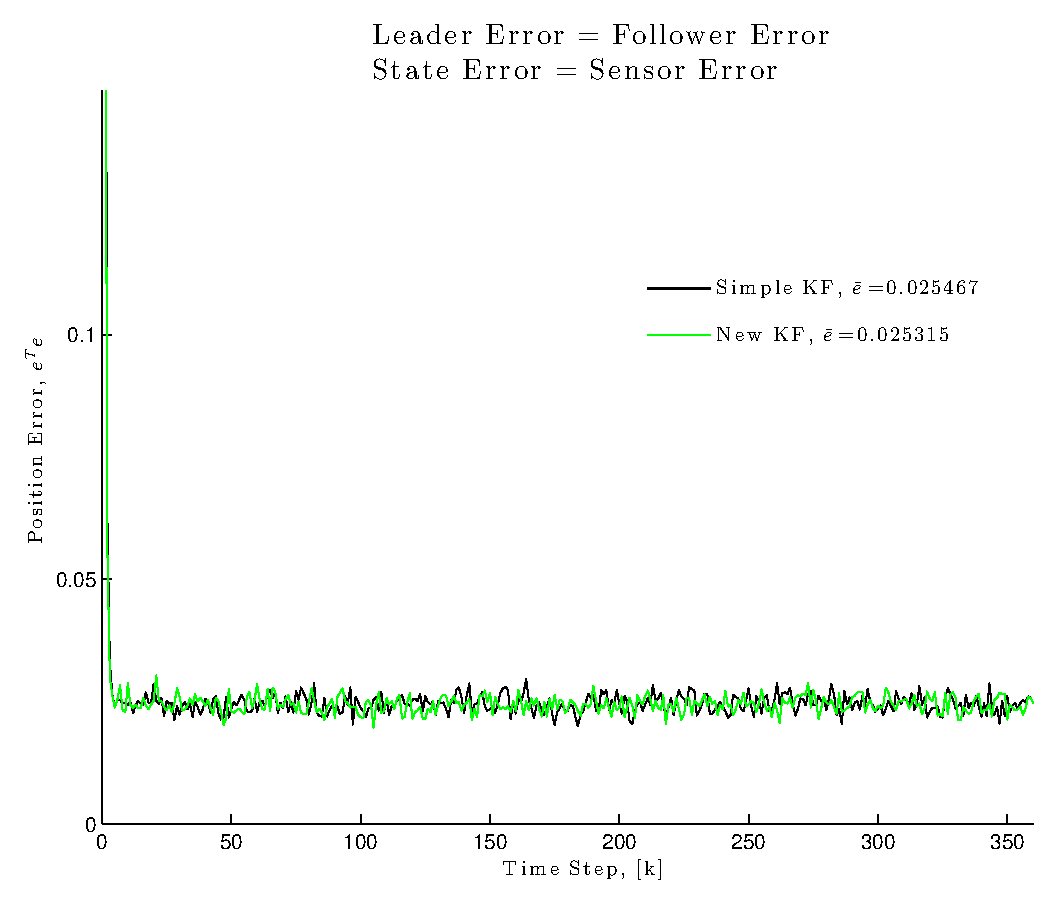
\includegraphics[scale=0.7]{fig1}
\end{figure}
\begin{figure}[!hbtp]
\centering
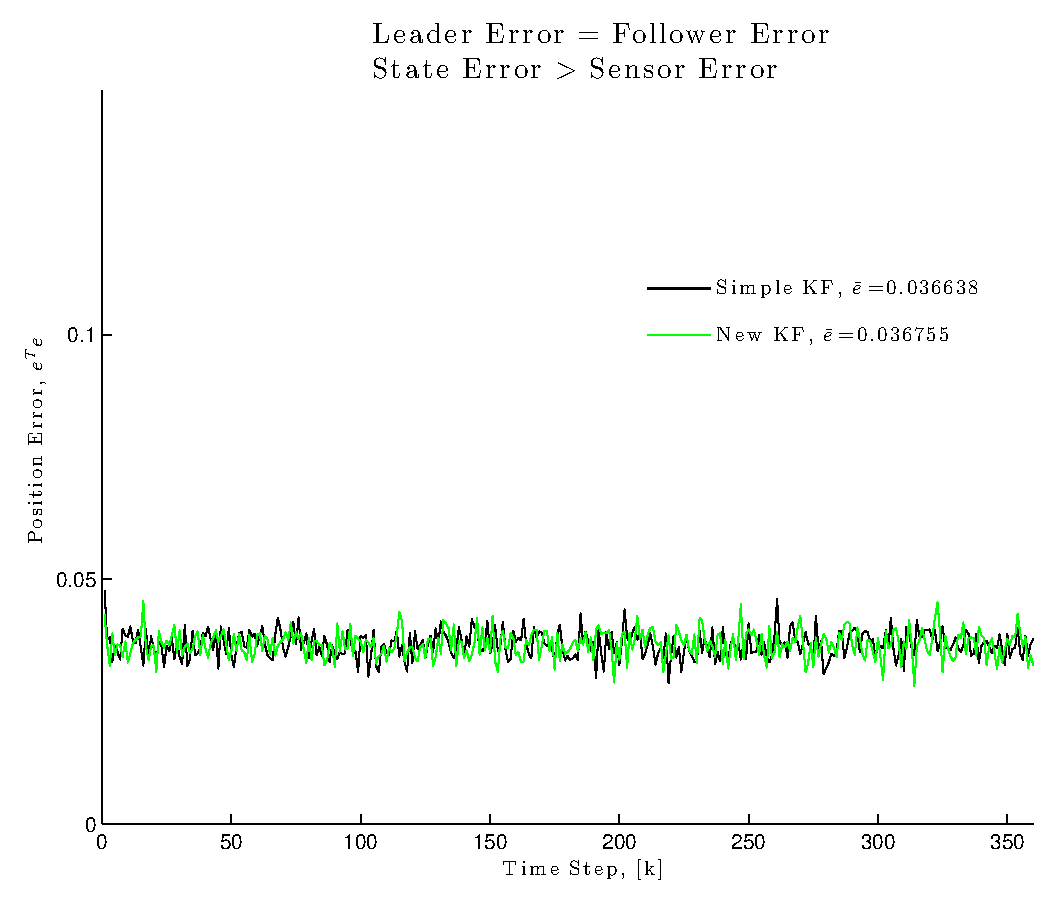
\includegraphics[scale=0.7]{fig2}
\end{figure}
\begin{figure}[!hbtp]
\centering
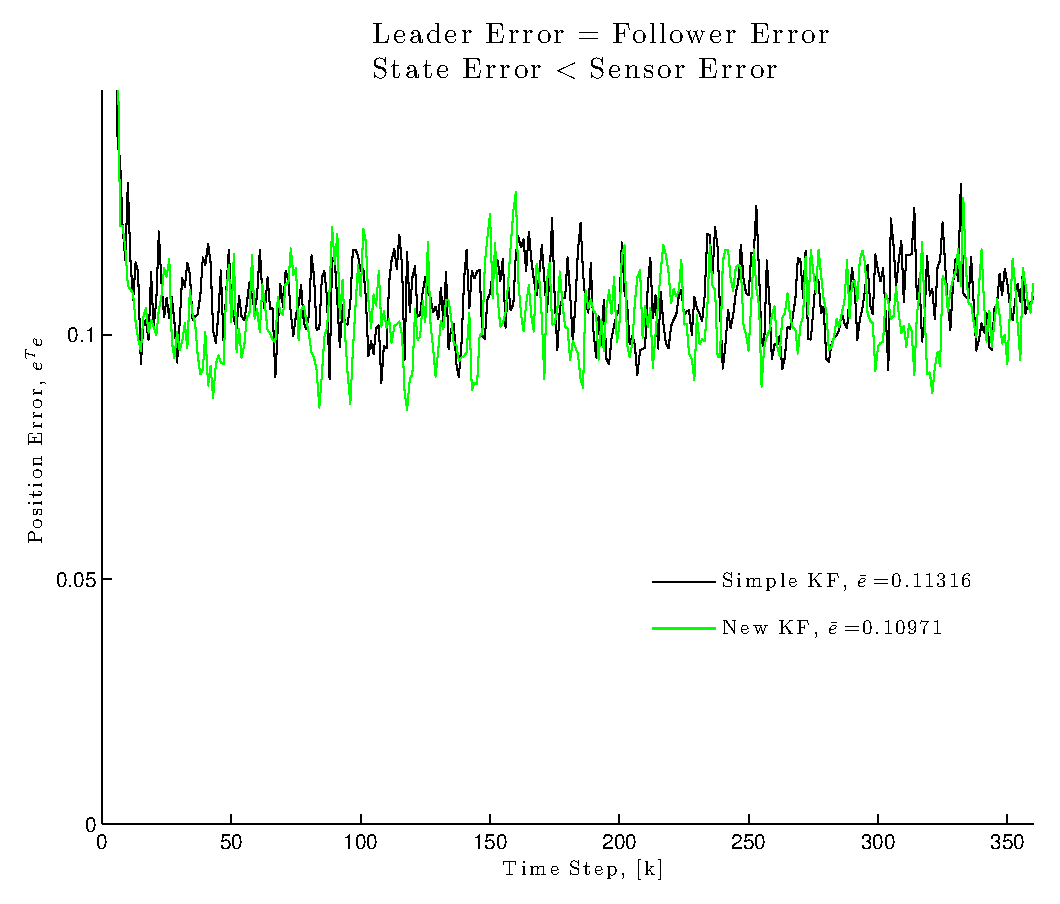
\includegraphics[scale=0.7]{fig3}
\end{figure}


\newpage

\section*{Section 2}
In the next three cases, the leader has larger error covariance matrices than the follower, so:
\begin{align*}
Q_{(l)} &= Q_{(f)} \times \gamma \\
R_{(l)} &= R_{(f)} \times \gamma \\
\text{where, } Q &: \text{state covariance error}\\
 R &: \text{sensor covariance error} \\
 \gamma &>1
\end{align*}
The cases that were tested in this section are:
\begin{itemize}
\item $Q_{(l)}=Q_{(f)}\times \gamma,$\\$R_{(l)}=R_{(f)}$
\item $Q_{(l)}=Q_{(f)},$\\ $R_{(l)}=R_{(f)} \times \gamma$
\item $Q_{(l)}=Q_{(f)} \times \gamma,$\\ $R_{(l)}=R_{(f)} \times \gamma$
\end{itemize}

\begin{figure}[!hbtp]
\centering
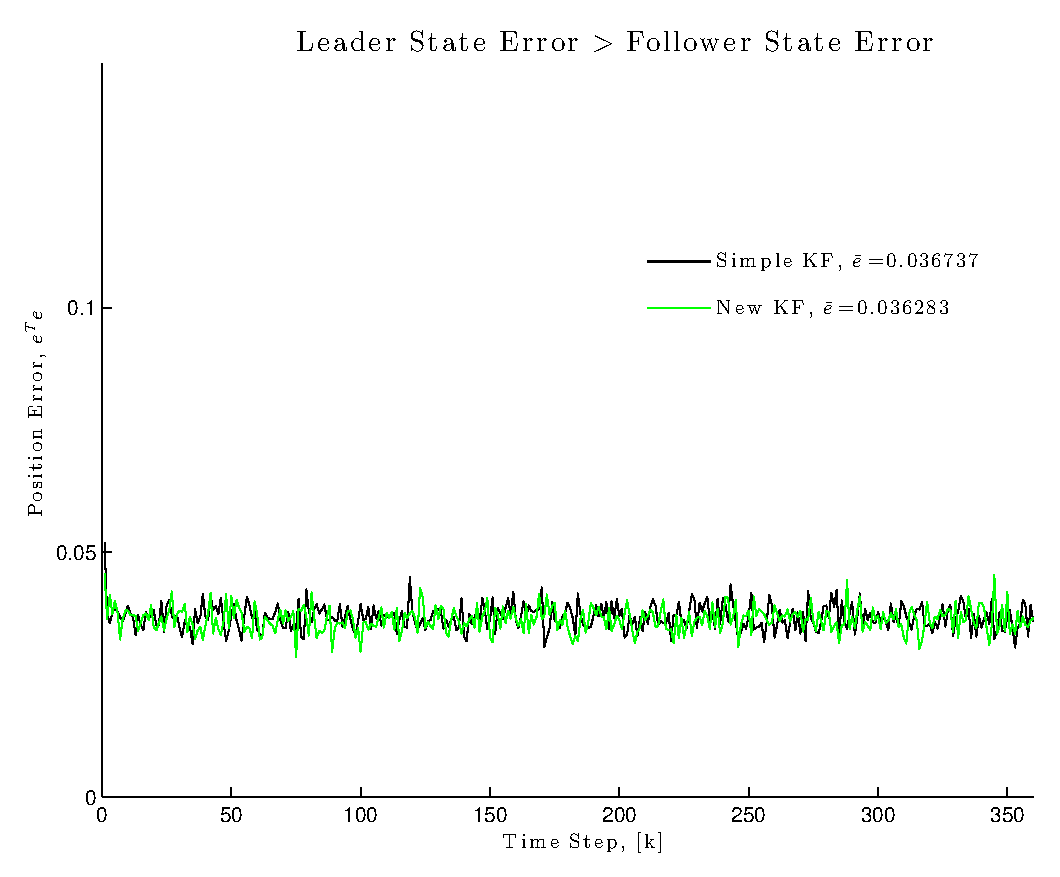
\includegraphics[scale=0.7]{fig4}
\end{figure}
\begin{figure}[!hbtp]
\centering
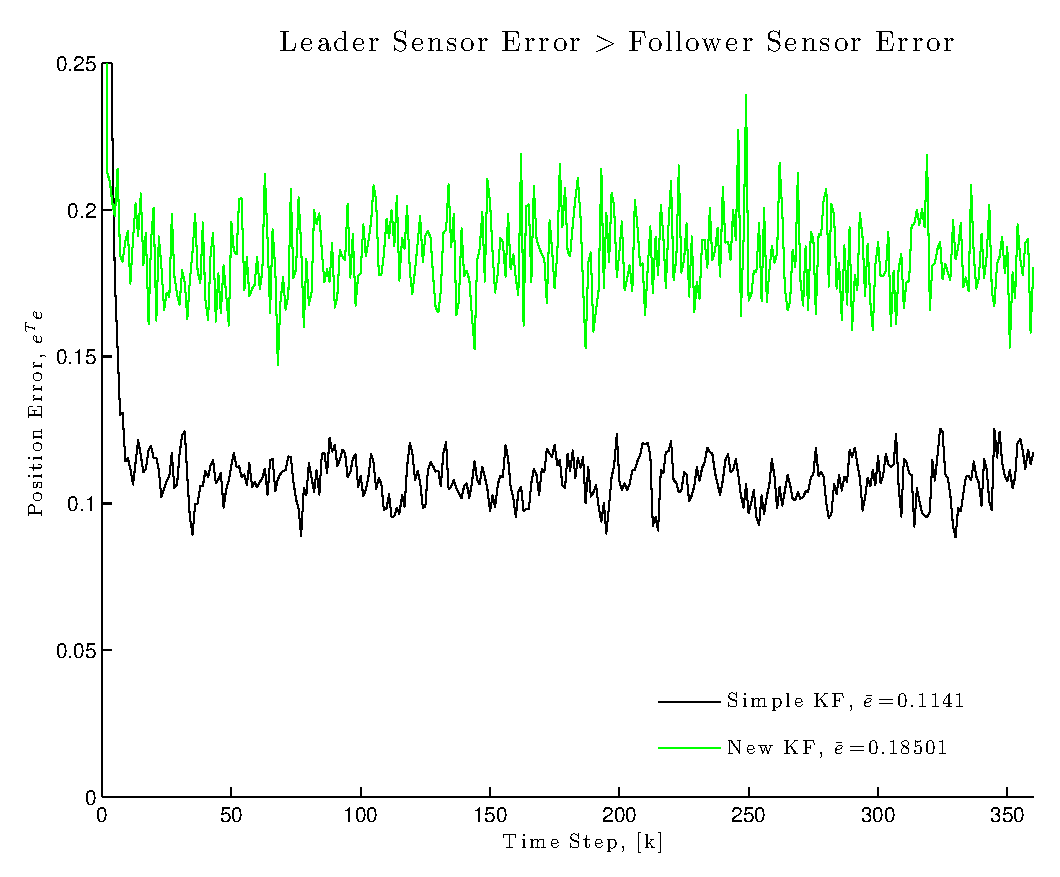
\includegraphics[scale=0.7]{fig5}
\end{figure}
\begin{figure}[!hbtp]
\centering
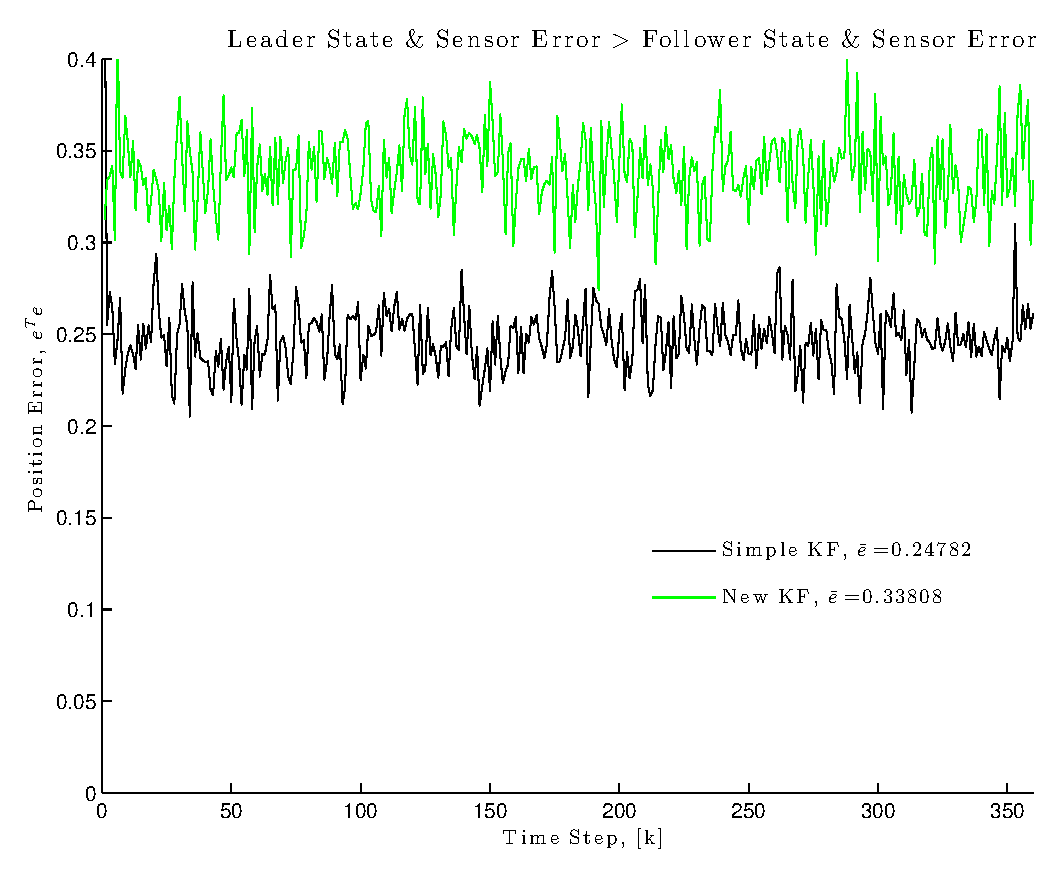
\includegraphics[scale=0.7]{fig6}
\end{figure}



\end{document}
